\chapter{Interactive Perception Library}
\label{chapter:Interactive Perception Library}


\section{Motivation and Goals}
Since we understand the world based on functionality and behavior, as a result, manipulation becomes an integral part of perception. In other words, purposeful manipulation depends on the robot's ability to curiously explore its unknown environment through interaction. Based on the increasing popularity of the interactive perception approach we created a common place that can unite researchers' efforts towards better algorithms and systems that concern adding manipulation in the perception loop. In addition to that, we developed a generic framework which can be of great help for sharing different implementations of similar problems. So far we received positive feedback from various institutes that decided to join the initiative, among others: Robotic Institute at Carnegie Mellon University, Robotics and Biology Laboratory at Technical University Berlin, Robotics Group at Robert Bosch LLC, Robotic Intelligence Laboratory at Universitat Jaume I. Having seen the success achieved by similar initiatives(e.g. openslam.org, opencv, pcl, etc.) we want to follow their footsteps in order to create a synergistic community of interactive perception researchers.

It is worth emphasising and it has been shown in the Chapter \ref{chapter:Related Work} that interactive perception field has gained many more potential applications than the ones presented in this thesis. These areas include interactive perception methods for object segmentation, modeling, grasping, and even learning manipulation skills through interactive perception. Interestingly, these results are beginning to appear independently in the different relevant communities: perception, grasping, manipulation, and learning.

Having this in mind we created a common, modular tool - Interactive Perception Library \footnote{\url{http://github.com/Lolu28/interactive_perception}} that can address researchers' needs to investigate interactive perception area more deeply and it can enable easier access to existing resources and algorithms. The main goal of this library is to collect all the code from different laboratories being involved in the idea of interactive perception. We developed a framework that enables to switch between different implementations of each module from the interactive perception pipeline at runtime. We decided to implement everything in Robot Operating System since it is easier to support various robots, include datasets and glue different algorithms together. 


\section{Library}
\subsection{Modules}
Looking at various systems created by different robotics institutes \todo{: REF} it can be noticed that there is a similar idea lying behind them.  

After conducting about research in existing implementations we noticed many similar modules that became crucial for our library, those being:

\begin{itemize}
\item Static Segmentation - to infer which parts of the scene are most likely being segmented incorrectly
\item Feature Extraction - to extract features that will be tracked
\item Push Point - to find the best point to interact with objects
\item Manipulation - to manipulate a robot in order to interact with objects in the scene
\item Tracker - to track previously extracted features during robot's movement
\item Trajectory Clustering - to cluster the trajectories of the features that have moved in the same manner
\item Full Reconstruction - to reconstruct a full model of the object. It takes the sparse representation - clustered features - and reconstructs a dense model of the object.
\end{itemize}

There are many reasons to motivate the choice of the pipeline we developed. Since the interactive perception systems use model-based approach, we incorporated feature extraction module. In order to improve robustness of algorithms we included the static segmentation module which works as a pre-processing step for our system. Having potential applications such as grasping and object recognition in mind, we included dense model reconstruction module.

The library was created based on the abstract factory pattern and it mainly uses pluginlib \footnote{\url{http://ros.org/wiki/pluginlib}} from ROS. The main executable shows a simple user interface together with a visualization tool(visualizer ROS package). The user interface shows possibility to call different modules and their particular implementations by using a simple GUI - dynamic reconfigure ROS package \footnote{\url{http://www.ros.org/wiki/dynamic_reconfigure}}. The details are described in the next section.

\subsection{Architecture}

In order to describe the architecture it is needed to explain the idea of the pluginlib library that was heavily used in this project. Pluginlib is a C++ library that enables to load and unload other classes (plugins) dynamically without being explicitly linked against their implementations. In this way pluginlib can open a library that it was not aware of before running the program. 

This tool gives us a number of possibilities that can be used in the Interactive Perception Library. Having in mind all the modules that we depicted in the previous sections we can dynamically switch between different implementations of each of these modules. For example, if we want to combine two different interactive perception algorithms we can just mix the modules from their pipeline by dynamically loading them. 

In addition to that, the library contains graphical debug tools that enable to check currently loaded point cloud as depicted in Figure \ref{fig:ipl}. It also provides the functionality of visualizing different outputs such as customized point types and point normals.

\begin{figure}
%\centering

{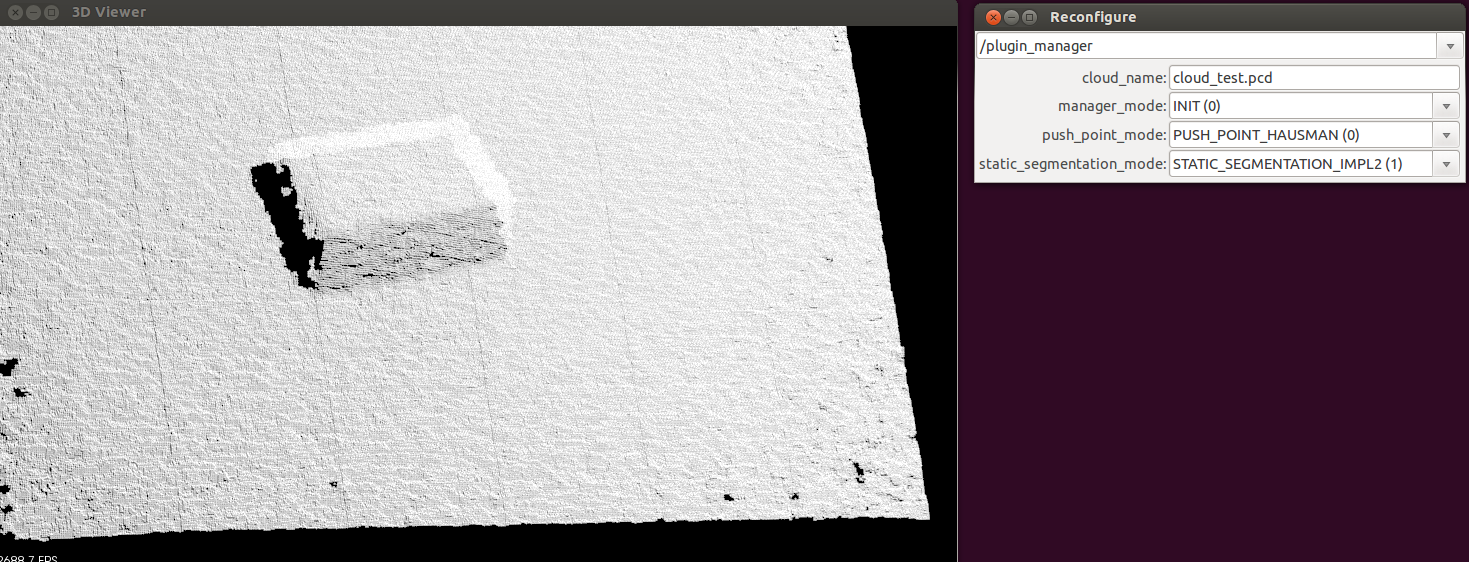
\includegraphics[width=1.1\columnwidth]{figures/ipl.png}}

\caption{Interactive Perception Library with running visualizer and a simple Graphical User Interface to choose the module and its implementation.}
\label{fig:ipl}
\end{figure}

The architecture is presented in Figure \ref{fig:uml}, in the form of an UML class diagram. There is a main class called PluginManager that is responsible for loading different plugins and executing respective steps of the algorithm. It delegates the visualization tasks to the class named Visualizer. The only connection that PluginManager has to the plugins is through the interactive perception interface ROS package that consists of all the interfaces for different modules. In addition to that, there are ROS packages holding an implementation of the respective module. In Figure \ref{fig:uml} there are two different implementations for two interfaces - StaticSegmentation and PushPointEstimation. The user can dynamically switch between PushPointImpl and PushPointImpl2 since both of them implement the same generic interface. This design enables other people to benchmark their modules against other algorithms and also to find the combination that fits best to their application.  

\begin{figure}
%\centering
{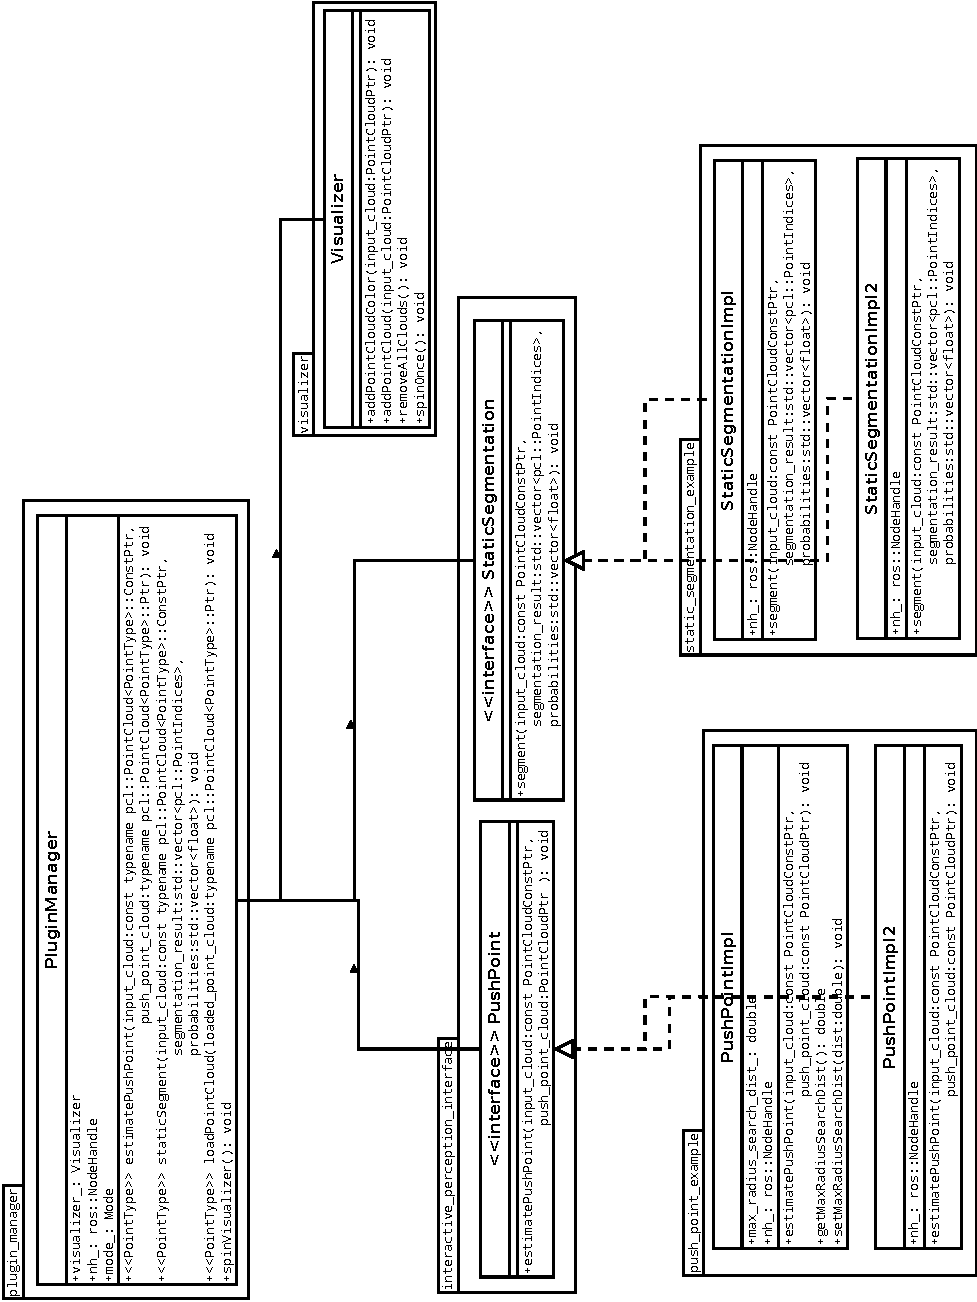
\includegraphics[width=0.9\columnwidth, angle=-90]{figures/uml-after.pdf}}

\caption{UML class diagram that shows the main structure of the library.}
\label{fig:uml}
\end{figure}




